% Esta sección describe equipo y procedimiento de manera simple.
% Reemplaza con tu propio contenido cuando enseñes o evalúes.

\subsection{Primer taller: Programación estructurada en sistemas embebidos} % Sub-sección metodológica

Este taller integrador se centra en el diseño y desarrollo de sistemas embebidos bajo el enfoque de la programación estructurada, integrando el modelado formal del sistema con su implementación práctica. A través de tres retos aplicados, el objetivo principal es desarrollar la capacidad de estructurar soluciones embebidas desde una perspectiva ingenieril, donde se debe justificar la selección del microcontrolador, organizar el código de forma modular y documentada, e implementar buenas prácticas en todo el desarrollo del mismo.

\subsubsection{RETO 1 – Sistema de Control de Acceso}\label{sec:reto1}
  

\begin{itemize}
    
    \item Análisis del problema:
    
     El sistema de control de acceso tiene como propósito verificar una contraseña digital ingresada mediante una combinación de botones físicos o un teclado matricial. Si la combinación es correcta, se activa una cerradura electrónica (servo motor o relé); en caso contrario, se contabilizan los intentos fallidos y, al superar el límite permitido, el sistema entra en un estado de bloqueo temporal.
     
        \begin{itemize}
             \item Identificación de Entradas y Salidas
                  \begin{itemize}       
                      \item Entradas del sistema:
                    
                            \begin{itemize}
                                 \item  Botones digitales (4 pulsadores) o teclado matricial 4x4 para ingreso de contraseña.

                                 \item Señal de reset (opcional): botón para reiniciar el sistema desde estado bloqueado.                      
                             \end{itemize}  
                             
                  \end{itemize}     

             \item Restricciones Técnicas
                     \begin{itemize}
                            \item Máximo 3 intentos fallidos antes de activar el bloqueo.
                            
                            \item Tiempo de bloqueo: 30 segundos.

                            \item La contraseña debe almacenarse en memoria no volátil (EEPROM) o en código.
                            
                            \item Temporización no bloqueante mediante millis()

                            \item El sistema debe retornar automáticamente al estado de espera tras el desbloqueo.
                     \end{itemize}
                     
             \item Variables Involucradas
                 
\begin{table}[h]
\centering
\caption{Variables del sistema de control de acceso}
\label{tab:Tabla_1_R1}
\footnotesize
\setlength{\tabcolsep}{4pt}
\renewcommand{\arraystretch}{1.5}
    
    \begin{tabularx}{\columnwidth}{|>{\raggedright\arraybackslash}p{3cm}|>{\centering\arraybackslash}p{1.5cm}|X|}
        \hline
        \textbf{Variable} & \textbf{Tipo} & \textbf{Descripción} \\
        
        \hline
        intentosFallidos & int & Contador de intentos incorrectos (0--3) \\ 
        
        \hline
        contrasenaIngresada & String & Secuencia de teclas presionadas por el usuario \\ 
        
        \hline
        contrasenaCorrecta & String & Contraseña almacenada en firmware \\ 
        
        \hline
        sistemaBloqueado & bool & Indica si el sistema está en estado de bloqueo \\ 
        
        \hline
        tiempoBloqueo & unsigned long & Marca de tiempo de inicio del bloqueo \\ 
        
        \hline
        accesoGarantizado & bool & Indicador de acceso concedido \\ \hline
\end{tabularx}
\end{table}
          
       \end{itemize}  
\end{itemize}


\begin{itemize}

       \item Flujograma del sistema
       
         A continuación se describe el algoritmo de comportamiento del sistema de control de acceso. El diagrama representa el flujo lógico completo desde el inicio hasta la resolución de cada evento de acceso.

             \begin{itemize}
             
                \item Descripción del Algoritmo (Pseudocódigo Estructurado):

                En el Algoritmo~\ref{alg:Algoritmo1} se puede observar el pseudocódigo, el cual, comienza declarando un bloque de INICIO que configura los periféricos. A continuación se evalúa si el sistema está bloqueado; en caso afirmativo, se verifica el temporizador y se libera al cumplirse 30 segundos. Si el sistema no está bloqueado, se espera la entrada del usuario. Cuando la contraseña está completa, se ejecuta la comparación: si es correcta, se activa el servo y el LED verde; si es incorrecta, se incrementa el contador de fallos y se evalúa si se alcanzó el límite. El proceso retorna al inicio del bucle en todos los casos.

                  
             \end{itemize}
             
\end{itemize}

\begin{algorithm}[h]
\caption{Algoritmo de Control de Acceso}
\label{alg:Algoritmo1}
\begin{algorithmic}[1]

\Statex \textbf{Inicialización:}
\State Inicializar pines, variables y servo en posición cerrada
\State $intentosFallidos = 0$
\State $sistemaBloqueado = false$

\While{true}

    \If{$sistemaBloqueado$}

        \If{$millis() - tiempoBloqueo \geq 30000$}
            \State $sistemaBloqueado = false$
            \State $intentosFallidos = 0$
            \State Apagar $LED\_ROJO$
        \EndIf

    \Else

        \State Leer tecla del teclado
        \State Agregar caracter a $contrasenaIngresada$

        \If{$|contrasenaIngresada| = |contrasenaCorrecta|$}

            \If{$contrasenaIngresada = contrasenaCorrecta$}

                \State Activar servo (abrir cerradura)
                \State Encender $LED\_VERDE$ durante 3 segundos
                \State Regresar servo a posicion cerrada
                \State $intentosFallidos = 0$

            \Else

                \State $intentosFallidos = intentosFallidos + 1$
                \State Hacer parpadear $LED\_ROJO$

                \If{$intentosFallidos \geq 3$}
                    \State $sistemaBloqueado = true$
                    \State $tiempoBloqueo = millis()$
                \EndIf

            \EndIf

            \State $contrasenaIngresada = " "$

        \EndIf

    \EndIf

\EndWhile

\end{algorithmic}
\end{algorithm} 
%\bigskip


\begin{itemize}

    \item Justificación técnica del microcontrolador seleccionado

        \begin{itemize}

             \item Microcontrolador Seleccionado: Arduino UNO (ATmega328P): El Arduino UNO con microcontrolador ATmega328P resulta adecuado para este sistema debido a su disponibilidad, bajo costo, amplia comunidad de soporte y suficiente cantidad de pines para los periféricos requeridos\cite{Arduino_datasheet}.

             \item Análisis de Pines Requeridos:
              El ATmega328P dispone de 14 pines digitales (6 con PWM) y 6 analógicos, cubriendo ampliamente los 12 pines requeridos con margen de expansión.
              
                 

\begin{table}[h]
\caption{Análisis de Pines Requeridos}
\label{tab:Tabla_2_R1}
\centering
\renewcommand{\arraystretch}{1.2}
\begin{tabular}{p{2.5cm} p{3.5cm} p{2cm}}
\toprule
\textbf{Componente} & \textbf{Pines Requeridos} & \textbf{Tipo} \\
\midrule
Teclado matricial 4x4 & 8 pines digitales (4 filas + 4 columnas) & Digital I/O \\
LED verde & 1 pin digital & Digital OUTPUT \\
LED rojo & 1 pin digital & Digital OUTPUT \\
Servo motor & 1 pin PWM & PWM OUTPUT \\
Buzzer & 1 pin digital & Digital OUTPUT \\
\midrule
\textbf{Total} & \textbf{12 pines} & --- \\
\bottomrule
\end{tabular}
\end{table}

             \item Capacidad de Procesamiento

                 \begin{itemize}
                 
                       \item CPU: ATmega328P @ 16 MHz
                       \item Memoria Flash: 32 KB (programa ocupa < 5 KB)
                       \item SRAM: 2 KB (suficiente para buffers de contraseña y variables de estado)
                       \item EEPROM: 1 KB (almacenamiento persistente de contraseña) 
                       
                 \end{itemize}

             \item Consumo Energético

                  \begin{itemize}
                 
                       \item Consumo activo: ~46 mA @ 5V = ~230 mW
                       \item LED: ~20 mA c/u con resistencia limitadora de 220 ohms
                       \item Servo SG90: ~100–250 mA en movimiento
                       \item Alimentación recomendada: 5V/1A (USB o adaptador)
                       
                 \end{itemize}
                 
             \item Componentes Auxiliares
                  \begin{table}[h]
\caption{Componentes Electrónicos del Sistema}
\label{tab:Tabla_3_R1}
\centering

\footnotesize
\setlength{\tabcolsep}{4pt}
\renewcommand{\arraystretch}{1.5}

\begin{tabularx}{\columnwidth}{|>{\raggedright\arraybackslash}p{3cm}|>{\centering\arraybackslash}p{1.5cm}|X|}
\hline
\textbf{Componente} & \textbf{Cant.} & \textbf{Especificación / Función} \\
\hline
LED verde 5mm & 1 & 3.3V, 20mA. Indicador de acceso correcto. \\
\hline
LED rojo 5mm & 1 & 3.3V, 20mA. Indicador de error o bloqueo. \\
\hline
Resistencia 220 $\Omega$ & 2 & 1/4 W. Limitación de corriente para los LEDs. \\
\hline
Buzzer pasivo & 1 & 5V. Generación de señal sonora de retroalimentación. \\
\hline
Protoboard / PCB & 1 & 830 puntos. Montaje físico del circuito. \\
\hline
\end{tabularx}

\end{table}

             \item Esquema de Conexión

             En la Figura \ref{fig:Imagen_1_R1} se observa el diagrama de conexión correspondiente al funcionamiento de este circuito, desarrollado a través del programa de circuitado. A continuación se mencionan las conexiones establecidas en el proyecto:
             \begin{itemize}
                 \item Teclado 4x4: Filas a pines D4, D5, D6, D7 — Columnas a pines D8, D9, D10, D11
                \item LED verde: Pin D12 → Resistencia 220 ohms → Ánodo LED → Cátodo → GND
                \item LED rojo: Pin D13 → Resistencia 220 ohms → Ánodo LED → Cátodo → GND
                \item Servo SG90: Cable señal a Pin D3 (PWM), VCC a 5V, GND a GND
                \item Buzzer: Pin D2 → Buzzer (+) → GND
                \item Alimentación: 5V desde USB o regulador 7805

             \end{itemize}
             \textit{EasyEDA}.
                  \begin{figure}[h]
                  \centering
                  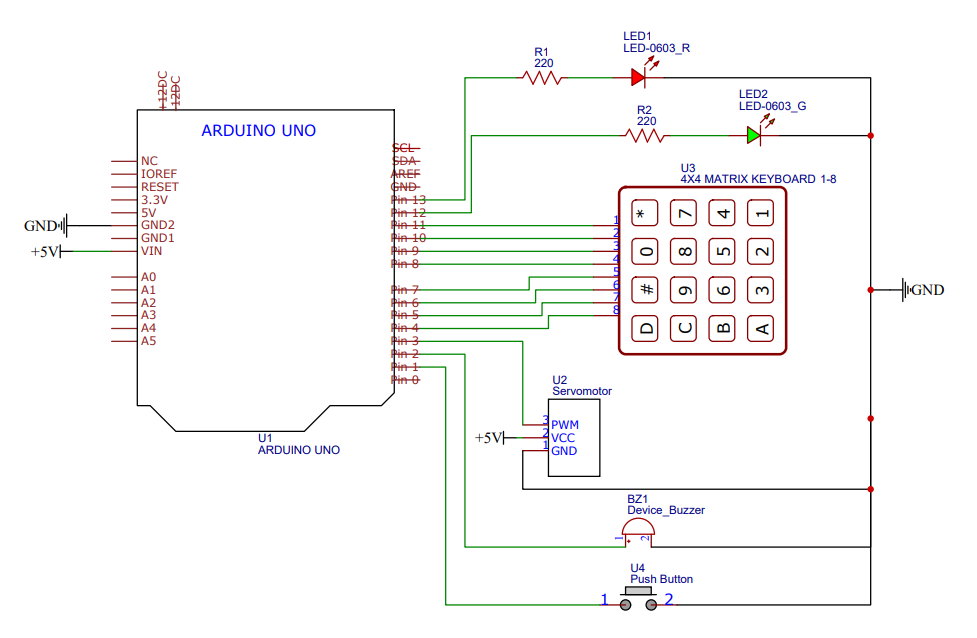
\includegraphics[width=\columnwidth]{images/Imagen_1R1.png}
                  \caption{Esquemático de Conexión Reto 1}
                  \label{fig:Imagen_1_R1}
                  \end{figure}
             
        \end{itemize}
  
\end{itemize}

\begin{itemize}
      \item Código documentado
      
      El código está organizado de forma modular separando la inicialización de hardware, la lógica de verificación, el control de la cerradura y la gestión de estados de bloqueo. Se evita el uso de delay() para garantizar temporización no bloqueante.

      \begin{lstlisting}[caption={Implementación de Control de Acceso con Teclado y Servo}, label={lst:control-acceso}]
#include <Keypad.h>
#include <Servo.h>

// --- Definicion de pines ---
#define PIN_SERVO       3
#define PIN_BUZZER      2
#define PIN_LED_VERDE   12
#define PIN_LED_ROJO    13
#define PIN_BOTON       A0

// --- Configuracion del teclado 4x4 ---
const byte FILAS    = 4;
const byte COLUMNAS = 4;

char teclas[FILAS][COLUMNAS] = {
  { '1', '2', '3', 'A' },
  { '4', '5', '6', 'B' },
  { '7', '8', '9', 'C' },
  { '*', '0', '#', 'D' }
};

byte pinesFilas[FILAS] =
  { 11, 10, 9, 8 };
byte pinesColumnas[COLUMNAS] =
  {  7,  6, 5, 4 };

Keypad teclado =
  Keypad(makeKeymap(teclas),
         pinesFilas,
         pinesColumnas,
         FILAS,
         COLUMNAS);

// --- Servo ---
Servo servo;
#define ANGULO_ABIERTO  90
#define ANGULO_CERRADO   0

// --- Variables de control de 
acceso ---
const String PASSWORD = "1234";
const byte MAX_INTENTOS = 3;
const unsigned long TIEMPO_BLOQUEO
= 30000;

// --- Estado general ---
String entradaActual = "";
byte intentosFallidos = 0;
bool bloqueado = false;
unsigned long tiempoBloqueo = 0;

// --- Servo temporizado ---
bool puertaAbierta = false;
unsigned long tiempoServo = 0;

// --- Buzzer no bloqueante ---
bool buzzerActivo = false;
unsigned long tiempoBeep = 0;
int duracionBeep = 0;

// --- Parpadeo LED rojo ---
unsigned long tiempoBlink = 0;
bool estadoBlink = false;
byte parpadeosPendientes = 0;
bool ledRojoFijo = false;

// --- Anti-rebote boton ---
unsigned long ultimoDebounce = 0;
const unsigned long 
DEBOUNCE_DELAY = 50;

// ===================
void inicializarHardware() {
  pinMode(PIN_LED_VERDE, OUTPUT);
  pinMode(PIN_LED_ROJO, OUTPUT);
  pinMode(PIN_BUZZER, OUTPUT);
  pinMode(PIN_BOTON, 
  INPUT_PULLUP);
  servo.attach(PIN_SERVO);
  servo.write(ANGULO_CERRADO);
  digitalWrite(PIN_LED_VERDE, LOW);
  digitalWrite(PIN_LED_ROJO,  LOW);
  Serial.println("Sistema de
  acceso listo");
}

// ===================
void beep(int frecuencia,
          int duracion) {
  tone(PIN_BUZZER, frecuencia);
  buzzerActivo = true;
  tiempoBeep   = millis();
  duracionBeep = duracion;
}

// ===================
void actualizarBuzzer() {
  if (buzzerActivo) {
    if (millis() - tiempoBeep
        >= duracionBeep) {
      noTone(PIN_BUZZER);
      buzzerActivo = false;
    }
  }
}

// ===================
void actualizarServo() {
  if (puertaAbierta) {
    if (millis() - tiempoServo
        >= 3000) {
      servo.write(ANGULO_CERRADO);
      digitalWrite(PIN_LED_VERDE,
      LOW);
      puertaAbierta = false;
    }
  }
}

// ===================
void actualizarBlink() {
  if (!estadoBlink) return;
  if (millis() - tiempoBlink < 300)
    return;
  tiempoBlink = millis();
  bool ledActual =
    digitalRead(PIN_LED_ROJO);
  if (!ledActual) {
    digitalWrite(PIN_LED_ROJO, HIGH);
    parpadeosPendientes--;
  } else {
    if (parpadeosPendientes == 0) {
      estadoBlink = false;
      digitalWrite(PIN_LED_ROJO,
        ledRojoFijo ? HIGH : LOW);
    } else {
      digitalWrite(PIN_LED_ROJO, LOW);
    }
  }
}

// ===================
void accesoAprobado() {
  intentosFallidos  = 0;
  estadoBlink       = false;
  ledRojoFijo       = false;
  digitalWrite(PIN_LED_ROJO,  LOW);
  digitalWrite(PIN_LED_VERDE, HIGH);
  servo.write(ANGULO_ABIERTO);
  puertaAbierta = true;
  tiempoServo   = millis();
  beep(2000, 150);
}

// ===================
void accesoNegado() {
  intentosFallidos++;
  if (intentosFallidos < 
  MAX_INTENTOS)
  {
    parpadeosPendientes = 2;
    ledRojoFijo         = false;
  } else {
    parpadeosPendientes = 3;
    ledRojoFijo         = true;
  }
  estadoBlink = true;
  tiempoBlink = millis();
  digitalWrite(PIN_LED_ROJO, LOW);
  beep(500, 500);
  if (intentosFallidos >= 
  MAX_INTENTOS)
  {
    bloqueado     = true;
    tiempoBloqueo = millis();
  }
}

// ===================
void verificarPassword() {
  if (entradaActual == PASSWORD)
    accesoAprobado();
  else
    accesoNegado();
  entradaActual = "";
}

// ===================
void procesarTecla(char tecla) {
  if (tecla == '#') {
    verificarPassword();
    return;
  }
  if (tecla == '*') {
    entradaActual = "";
    beep(1000, 100);
    return;
  }
  entradaActual += tecla;
  if (entradaActual.length()
      > PASSWORD.length()) {
    entradaActual = "";
    beep(500, 200);
  }
}

// ===================
void leerBoton() {
  if (digitalRead(PIN_BOTON) == LOW) {
    if (millis() - ultimoDebounce
        > DEBOUNCE_DELAY) {
      bloqueado        = false;
      intentosFallidos = 0;
      entradaActual    = "";
      estadoBlink      = false;
      ledRojoFijo      = false;
      digitalWrite(PIN_LED_ROJO, LOW);
      digitalWrite(PIN_LED_VERDE, 
      LOW);
      beep(1800, 200);
      ultimoDebounce = millis();
    }
  }
}

// ===================
void setup() {
  Serial.begin(9600);
  inicializarHardware();
}

// ===================
void loop() {
  actualizarBuzzer();
  actualizarServo();
  actualizarBlink();
  leerBoton();
  if (bloqueado) {
    if (millis() - tiempoBloqueo
        >= TIEMPO_BLOQUEO) {
      bloqueado        = false;
      intentosFallidos = 0;
      estadoBlink      = false;
      ledRojoFijo      = false;
      digitalWrite(PIN_LED_ROJO, LOW);
      beep(1500, 300);
    }
    return;
  }
  char tecla = teclado.getKey();
  if (tecla) procesarTecla(tecla);
}
\end{lstlisting}
      
\end{itemize}




\subsubsection{RETO 2 – Sistema de Control de Acceso}\label{sec:reto2}
  \begin{itemize}
    \item Análisis del problema
        \begin{itemize}
        
            \item Descripción general:
            El sistema de monitoreo con alarmas supervisa continuamente una variable física y clasifica su valor en tres niveles operativos: Normal, Advertencia y Crítico. Para cada nivel se activan indicadores visuales y/o sonoros diferenciados. Se implementa histéresis para evitar oscilaciones inestables en los umbrales de transición.

        \end{itemize} 

    \item Identificación de Entradas y Salidas
        \begin{itemize}
            
            \item Entradas:
                \begin{itemize}
                    \item  Sensor de temperatura (señal analógica o digital).

                    \item Botón de silencio de alarma (opcional).                   
                \end{itemize}
            
            \item Salidas:
                \begin{itemize}
                    \item  LED verde: estado Normal.
                    
                    \item LED amarillo: estado Advertencia.    
                    \item LED rojo: estado Crítico. 

                    \item Buzzer: alarma sonora en Advertencia y Crítico.
                    
                \end{itemize}

    \item Restricciones técnicas
        \begin{itemize}
            \item Los umbrales deben ser configurables mediante constantes.

            \item Implementación obligatoria de histéresis para evitar inestabilidad en los límites.
            
            \item El sistema debe funcionar en ciclo continuo con temporización no bloqueante.
            
            \item La lectura del sensor debe ser promediada para reducir ruido.
            
        \end{itemize}
       
    \item Definición de umbrales y variables:

    En la Tabla~\ref{tab:Tabla_1_R2}, se observa la definición de las variables con sus respectivas descripciones y justificación. Reconocer las variables a utilizar sera de ayuda a la hora de realizar el código.

    

\begin{table}[!ht]
\centering
\caption{Definición de Umbrales y Variables}
\label{tab:Tabla_1_R2}
\footnotesize
\setlength{\tabcolsep}{3pt}
\renewcommand{\arraystretch}{1.3}
    \begin{tabularx}{\columnwidth}{|p{3.2cm}|p{2cm}|X|}

        \hline
        \textbf{Variable} & \textbf{Valor} & \textbf{Descripción} \\ 

        \hline UMBRAL\_ADVERTENCIA & const = 30°C & Umbral para activar advertencia \\ 

        \hline UMBRAL\_CRITICO & const = 40°C & Umbral para nivel crítico \\ 

        \hline HISTERESIS & const = 2°C & Margen para evitar fluctuaciones \\ 

        \hline temperaturaActual & float & Valor del sensor en °C \\ 

        \hline estadoActual & enum & NORMAL, ADVERTENCIA, CRÍTICO \\ 
    
        \hline tiempoUltimaLectura & unsigned long & Timestamp de la lectura \\ 
        
        \hline
    \end{tabularx}
\end{table}

    \item Flujograma del Sistema

    El algoritmo, que se observa como Algoritmo ~\ref{alg:control_temp},
    funciona en ciclo continuo, e implementa un sistema de monitoreo de temperatura basado en una máquina de estados con tres niveles: NORMAL, ADVERTENCIA y CRÍTICO. Cada 500 ms se realiza una nueva lectura del sensor, se calcula la temperatura y se determina el estado del sistema aplicando histéresis. En función del estado, se activan los indicadores correspondientes.
    
    

\begin{algorithm}[t]
\caption{Control de Temperatura con Histéresis}
\label{alg:control_temp}
\begin{algorithmic}[1]

\Statex \textbf{INICIO}
\State Inicializar pines, LCD, sensor
\State $\text{estadoActual} \gets \text{NORMAL}$

\Loop \ \textbf{PRINCIPAL} (cada 500 ms)
    \State $\text{temperaturaActual} \gets \text{leerSensor}()$
    
    \If{$\text{estadoActual} = \text{NORMAL}$}
        \If{$\text{temperaturaActual} \geq \text{UMBRAL\_ADVERTENCIA}$}
            \State $\text{estadoActual} \gets \text{ADVERTENCIA}$
        \EndIf

    \ElsIf{$\text{estadoActual} = \text{ADVERTENCIA}$}
        \If{$\text{temperaturaActual} \geq \text{UMBRAL\_CRITICO}$}
            \State $\text{estadoActual} \gets \text{CRITICO}$
        \ElsIf{$\text{temperaturaActual} < (\text{UMBRAL\_ADVERTENCIA} - \text{HISTERESIS})$}
            \State $\text{estadoActual} \gets \text{NORMAL}$
        \EndIf

    \ElsIf{$\text{estadoActual} = \text{CRITICO}$}
        \If{$\text{temperaturaActual} < (\text{UMBRAL\_CRITICO} - \text{HISTERESIS})$}
            \State $\text{estadoActual} \gets \text{ADVERTENCIA}$
        \EndIf
    \EndIf

    \State actualizarIndicadores($\text{estadoActual}$)
    \State mostrarEnLCD($\text{temperaturaActual, estadoActual}$)
\EndLoop
\Statex \textbf{FIN}

\end{algorithmic}
\end{algorithm}

    \item Justificación técnica del microcontrolador
        \begin{itemize}
            \item Microcontrolador Seleccionado: Arduino UNO (ATmega328P)

            El mismo microcontrolador del reto anterior es suficiente para este segundo reto.  Para usar el DHT21, se requiere únicamente un pin digital con protocolo one-wire.

            \item Análisis de Pines Requeridos:

            En la Tabla~\ref{tab:Tabla_2_R2}, se observan los pines solicitados para el correcto funcionamiento del programa.

            
\begin{table}[ht]
\caption{Análisis de Pines Requeridos (Sistema de Monitoreo)}
\label{tab:Tabla_2_R2}
\centering
\renewcommand{\arraystretch}{1.3}
\begin{tabularx}{\columnwidth}{X p{2.0cm} p{2.0cm}}
\toprule
\textbf{Componente} & \textbf{Pin} & \textbf{Tipo} \\
\midrule
Sensor NTC / DHT21 & A0 o D2 & Analógico / Digital \\
LED verde & D9 & Digital OUTPUT \\
LED amarillo & D10 & Digital OUTPUT \\
LED rojo & D11 & Digital OUTPUT \\
Buzzer & D8 & Digital OUTPUT \\

\midrule
\textbf{Total} & \textbf{6 pines} & --- \\
\bottomrule
\end{tabularx}
\end{table}

            \item Componentes auxiliares

            El sistema emplea como elemento principal de medición un sensor de temperatura DHT21. La visualización de la información se realiza mediante monitor serial en el Arduino IDE, lo que optimiza el uso de pines del microcontrolador.
            
            Para la señalización del estado del sistema se utilizan tres LEDs de 5 mm (verde, amarillo y rojo) de 20 mA, cada uno con su respectiva resistencia limitadora de 220 ohms para protección. Además, se integra un buzzer activo de 5 V y aproximadamente 85 dB que funciona como alarma sonora en condiciones críticas, reforzando la advertencia al usuario.

            \item Esquema de conexión 

            En la Figura \ref{fig:Imagen_1R2} se observa el diagrama de conexión correspondiente al funcionamiento de este circuito, desarrollado a través del programa de circuitado. A continuación se mencionan las conexiones realizadas:
            \begin{itemize}
                \item Sensor DHT21: D2 → pin DATA (resistencia pull-up 10k ohms entre DATA y VCC), VCC a 5V, GND a GND
                \item LED verde: D9 → 220 ohms → LED → GND
                \item LED amarillo: D10 → 220 ohms → LED → GND
                \item LED rojo: D11 → 220 ohms → LED → GND
                \item Buzzer: D8 → buzzer (+) → GND
            \end{itemize}
            \textit{EasyEDA}.
                  \begin{figure}[h]
                  \centering
                  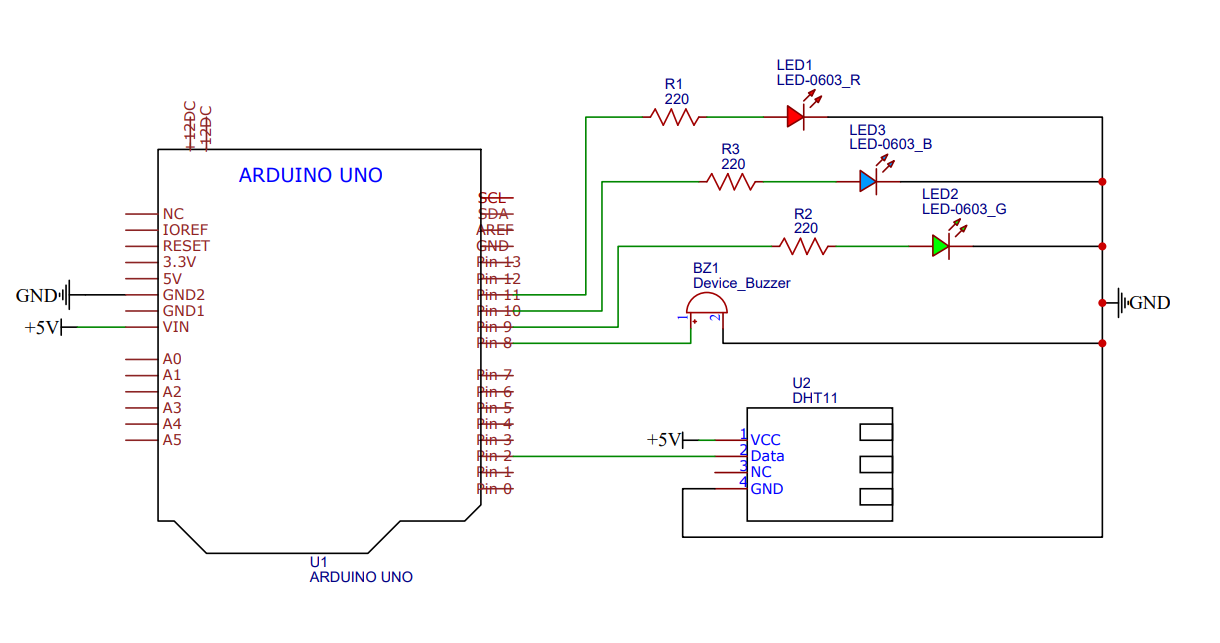
\includegraphics[width=\columnwidth]{images/Imagen_1R2.png}
                  \caption{Esquemático de Conexión Reto 2}
                  \label{fig:Imagen_1R2}
                  \end{figure}
            
        \end{itemize}

    \item Código Documentado

    El código propuesto documentado se encuentra registrado a continuación:
    \begin{lstlisting}[caption={Sistema de Monitoreo de Temperatura con DHT11}, label={lst:monitoreo-temperatura}]
#include <DHT.h>

// --- Pines ---
const int PIN_SENSOR       = 2;
const int PIN_LED_VERDE    = 9;
const int PIN_LED_AMARILLO = 10;
const int PIN_LED_ROJO     = 11;
const int PIN_BUZZER       = 8;

// --- Configuracion DHT11 ---
#define DHTTYPE DHT11
DHT dht(PIN_SENSOR, DHTTYPE);

// --- Umbrales de temperatura ---
const float UMBRAL_ADVERTENCIA = 30.0;  
const float UMBRAL_CRITICO     = 40.0;  
const float HISTERESIS         = 2.0;   

// --- Enumeracion de estados ---
enum EstadoSistema 
{ NORMAL, ADVERTENCIA, CRITICO };
EstadoSistema estadoActual = NORMAL;

// --- Variables de temporizacion ---
unsigned long tiempoUltimaLectura = 0;
const long    INTERVALO_LECTURA   = 2000;
unsigned long tiempoBuzzer        = 0;
bool          estadoBuzzer        = false;

float leerTemperatura() {
  float temp = dht.readTemperature();
  if (isnan(temp)) {
    Serial.println("Error al leer 
    el DHT11");
    return -999.0;
  }
  return temp;
}

void evaluarEstado(float temperatura) {
  if (temperatura == -999.0) return;
  switch (estadoActual) {
    case NORMAL:
      if (temperatura >= 
      UMBRAL_ADVERTENCIA)
        estadoActual = ADVERTENCIA;
      break;
    case ADVERTENCIA:
      if (temperatura >= UMBRAL_CRITICO)
        estadoActual = CRITICO;
      else if (temperatura < 
               UMBRAL_ADVERTENCIA 
               - HISTERESIS)
        estadoActual = NORMAL;
      break;
    case CRITICO:
      if (temperatura < UMBRAL_CRITICO 
      - HISTERESIS)
        estadoActual = ADVERTENCIA;
      break;
  }
}

void actualizarLEDs() {
  digitalWrite(PIN_LED_VERDE,
               estadoActual == NORMAL);
  digitalWrite(PIN_LED_AMARILLO,
               estadoActual == 
               ADVERTENCIA);
  digitalWrite(PIN_LED_ROJO,
               estadoActual == 
               CRITICO);
}

void gestionarBuzzer() {
  if (estadoActual == NORMAL) {
    noTone(PIN_BUZZER);
    return;
  }
  long intervalo = 
    (estadoActual == ADVERTENCIA)
    ? 1000 : 250;
  if ((millis() - tiempoBuzzer)
  >= intervalo) {
    tiempoBuzzer = millis();
    estadoBuzzer = !estadoBuzzer;
    if (estadoBuzzer)
      tone(PIN_BUZZER, 1500,
      intervalo / 2);
    else
      noTone(PIN_BUZZER);
  }
}

void setup() {
  Serial.begin(9600);
  dht.begin();
  pinMode(PIN_LED_VERDE,    OUTPUT);
  pinMode(PIN_LED_AMARILLO, OUTPUT);
  pinMode(PIN_LED_ROJO,     OUTPUT);
  pinMode(PIN_BUZZER,       OUTPUT);
  Serial.println("Sistema de 
  Monitoreo - Activo");
}

void loop() {
  unsigned long ahora = millis();
  if (ahora - tiempoUltimaLectura >= 
      INTERVALO_LECTURA) {
    tiempoUltimaLectura = ahora;
    float temperatura = leerTemperatura();
    evaluarEstado(temperatura);
    actualizarLEDs();
    Serial.print("T=");
    Serial.print(temperatura);
    Serial.print(" Estado=");
    Serial.println(estadoActual);
  }
  gestionarBuzzer();
}
\end{lstlisting}


    
    \end{itemize}  
\end{itemize}


\subsubsection{RETO 3 – Sistema de Control de Acceso}\label{sec:reto3}
  \begin{itemize}
    \item Análisis del problema
        \begin{itemize}
        
            \item Descripción general:
            El sistema de riego automático para cultivo de tomate monitorea continuamente la humedad relativa del ambiente mediante un sensor digital DHT11. Cuando la humedad desciende por debajo de un umbral mínimo, activa una bomba de agua (mediante relé) para iniciar el riego. El proceso se detiene al alcanzar el nivel de humedad óptimo. Se implementa histéresis para evitar ciclos de encendido/apagado rápidos y temporización no bloqueante para garantizar un funcionamiento secuencial estable. La información del sistema se visualiza en una pantalla OLED I2C de 0.96".

        \end{itemize} 

        \item Identificación de Entradas y Salidas
        \begin{itemize}
            
            \item Entradas:
                \begin{itemize}
                    \item  Sensor DHT11: señal digital en pin D2 (humedad relativa y temperatura).

                    \item Botón de riego manual (override): pin digital D3.                  
                \end{itemize}
            
            \item Salidas:
                \begin{itemize}
                    \item Módulo relé 5V: activa/desactiva la bomba de agua.
                    \item LED verde: humedad adecuada (IDLE).    
                    \item LED azul/amarillo: riego activo (REGANDO).
                    \item LED rojo: humedad crítica baja (ALARMA).
                    \item Pantalla OLED I2C 0.96" 128x64: visualización del porcentaje de humedad y estado del sistema.
                \end{itemize}
        \end{itemize}

        \item Restricciones técnicas
            \begin{itemize}
                \item No se debe usar delay() en el ciclo principal.
                \item Implementación de histéresis en umbrales de humedad.
                \item El sistema debe operar de forma completamente autónoma sin intervención humana.
                \item Separación de la lógica de negocio del control de hardware.
                \item El DHT11 requiere un intervalo mínimo de 2000 ms entre lecturas.
                \item Tiempo mínimo de riego: 5 segundos para evitar micro-ciclos.
                
            \end{itemize}

        \item Definición de umbrales y variables:

        En la Tabla~\ref{tab:Table_1_R3}, se observa la definición de las variables con sus respectivas descripciones y justificación. Reconocer las variables a utilizar sera de ayuda a la hora de realizar el código.

        \begin{table}[ht]
\caption{Variables Involucradas (Sistema de Riego Automático)}
\label{tab:Table_1_R3}
\centering
\renewcommand{\arraystretch}{1.3}
\begin{tabularx}{\columnwidth}{X p{2.0cm} p{2.0cm}}
\toprule
\textbf{Variable} & \textbf{Tipo} & \textbf{Valor / Rango} \\
\midrule
UMBRAL\_SECO   & const int    & 30\%       \\
UMBRAL\_HUMEDO & const int    & 70\%       \\
UMBRAL\_ALARMA & const int    & 20\%       \\
HISTERESIS     & const int    & 5\%        \\
humedadActual  & float        & 0--100\%   \\
estadoRiego    & enum         & IDLE / REGANDO / ALARMA \\
bombaActiva    & bool         & true / false \\
tiempoInicioRiego & unsigned long & ms      \\
tiempoMinRiego & const long   & 5000 ms    \\
\midrule
\textbf{Total} & \textbf{9 variables} & --- \\
\bottomrule
\end{tabularx}
\end{table}

        \item Flujograma del Sistema

        El sistema opera mediante un ciclo continuo con lecturas periódicas del sensor DHT11 cada 2000 ms. La lógica de control de la bomba se ejecuta basándose en el estado actual y los valores de humedad medidos, aplicando histéresis para garantizar estabilidad.

        \begin{algorithm}[ht]
\caption{Algoritmo de Sistema de Riego Automático}
\label{alg:Algoritmo_Riego}
\begin{algorithmic}[1]
\Statex \textbf{Inicialización:}
\State Inicializar pines, YI69, relé en OFF y pantalla OLED
\State $estadoRiego = IDLE$
\State $bombaActiva = false$
\While{true}
    \If{$millis() - tiempoUltimaLectura \geq 2000$}
        \State $tiempoUltimaLectura = millis()$
        \State $humedadActual = dht.readHumidity()$
        \If{$humedadActual = invalida$}
            \State Mostrar error en OLED
        \Else
            \If{$estadoRiego = IDLE$}
                \If{$humedadActual < UMBRAL\_ALARMA$}
                    \State $estadoRiego = ALARMA$
                    \State $activarBomba()$
                \ElsIf{$humedadActual \leq UMBRAL\_SECO$}
                    \State $estadoRiego = REGANDO$
                    \State $activarBomba()$
                    \State $tiempoInicioRiego = millis()$
                \EndIf
            \ElsIf{$estadoRiego = REGANDO$}
                \If{$millis() - tiempoInicioRiego \geq tiempoMinRiego$}
                    \If{$humedadActual \geq UMBRAL\_HUMEDO$}
                        \State $estadoRiego = IDLE$
                        \State $desactivarBomba()$
                    \EndIf
                \EndIf
            \ElsIf{$estadoRiego = ALARMA$}
                \State $activarBomba()$
                \If{$humedadActual \geq (UMBRAL\_SECO + HISTERESIS)$}
                    \State $estadoRiego = IDLE$
                    \State $desactivarBomba()$
                \EndIf
            \EndIf
            \State $actualizarIndicadores(estadoRiego)$
            \State $mostrarP(humedadActual,\ estadoRiego)$
        \EndIf
    \EndIf
    \State $gestionarBuzzerAlarma()$
    \State $verificarBotonManual()$
\EndWhile
\end{algorithmic}
\end{algorithm}

        \item Justificación técnica del microcontrolador
            \begin{itemize}
                \item Microcontrolador Seleccionado: Arduino UNO (ATmega328P)
    
                Para el sistema de riego autónomo se selecciona el Arduino UNO. El ATmega328P es suficiente para este prototipo educativo dado que el DHT11 utiliza un único pin digital y la pantalla OLED SSD1306 se comunica por I2C, ocupando únicamente los pines A4 y A5. Para aplicaciones de campo se recomendaría el Arduino Nano o ESP32 por su menor consumo energético y posibilidad de conectividad inalámbrica.
    
                \item Análisis de Pines Requeridos:
    
                En la Tabla~\ref{tab:Tabla_2_R3}, se observan los pines solicitados para el correcto funcionamiento del programa.
    
                \begin{table}[ht]
\caption{Análisis de Pines Requeridos (Sistema de Riego Automático)}
\label{tab:Tabla_2_R3}
\centering
\renewcommand{\arraystretch}{1.3}
\begin{tabularx}{\columnwidth}{p{2.2cm} p{1.0cm} p{1.5cm} X}
\toprule
\textbf{Componente} & \textbf{Pin} & \textbf{Tipo} & \textbf{Descripción} \\
\midrule
Sensor DHT11        & D2    & Digital IN  & Lectura de humedad relativa y temperatura \\
Módulo relé 5V      & D4    & Digital OUT & Control de bomba de agua \\
LED verde (IDLE)    & D5    & Digital OUT & Estado normal \\
LED azul (REGANDO)  & D6    & Digital OUT & Estado de riego activo \\
LED rojo (ALARMA)   & D7    & Digital OUT & Estado de alarma \\
Buzzer              & D8    & Digital OUT & Alarma sonora \\
Botón manual        & D3    & Digital IN  & Detención manual del riego \\
OLED SSD1306 0.96'' & A4/A5 & I2C         & Visualización del sistema \\
\midrule
\textbf{Total} & \textbf{8 pines} & --- & --- \\
\bottomrule
\end{tabularx}
\end{table}

                \item Capacidad de Procesamiento y Consumo
                \begin{itemize}
                    \item CPU: ATmega328P @ 16 MHz — suficiente para lectura digital y control.

                    \item Consumo sistema: ~85 mA (sin bomba); el DHT11 consume ~1 mA y la OLED ~20 mA en operación.

                    \item Relé 5V: bobina ~70 mA; la bomba se alimenta de fuente externa.

                    \item Se recomienda fuente de 12V/2A para alimentar tanto el Arduino como la bomba.

                    \item El relé desacopla galvánicamente el microcontrolador de la carga.
                \end{itemize}
    
                \item Componentes auxiliares
    
                En la tabla \ref{tab:Tabla_3_R3}, se observan los componentes relevantes al proyecto a desarrollar.

                \begin{table}[ht]
\caption{Componentes Auxiliares (Sistema de Riego Automático)}
\label{tab:Tabla_3_R3}
\centering
\renewcommand{\arraystretch}{1.3}
\begin{tabularx}{\columnwidth}{p{2.2cm} p{2.0cm} X}
\toprule
\textbf{Componente} & \textbf{Especificación} & \textbf{Función} \\
\midrule
Sensor DHT11
  & Digital, 3.3--5V, $\pm$5\% HR
  & Medición de humedad relativa del ambiente \\
Módulo relé 1 canal 5V
  & Carga máx. 10A / 250VAC
  & Conmutación de la bomba de agua \\
Mini bomba de agua 5V
  & 120 L/h, 0.5--1.2W
  & Suministro de agua al cultivo \\
Tubería de silicona 6mm
  & ---
  & Conducción del agua \\
LEDs 5mm (verde, rojo, azul)
  & 20 mA c/u
  & Indicadores visuales de estado \\
Resistencias 220$\Omega$
  & 3 unidades
  & Limitación de corriente para LEDs \\
OLED SSD1306 0.96''
  & I2C, 128x64 px, $\sim$20mA
  & Visualización de datos en tiempo real \\
Fuente 12V / 2A
  & DC regulada
  & Alimentación del sistema completo \\
\bottomrule
\end{tabularx}
\end{table}
    
                \item Esquema de conexión 
                En la Figura \ref{fig:Imagen_1R3} se observa el diagrama de conexión correspondiente al funcionamiento de este circuito, desarrollado a través del programa de circuitado. A continuación, se mencionan los pines conectados.
                \begin{itemize}
                    
                    \item DHT11: pin DATA a D2, VCC a 5V, GND a GND 
                
                    \item Relé: IN a pin D4, VCC a 5V, GND a GND; bornes COM/NO a bomba y fuente externa

                    \item LED verde: D5 → 220 ohms → LED → GND

                    \item LED azul: D6 → 220 ohms → LED → GND

                    \item LED rojo: D7 → 220 ohms → LED → GND

                    \item Buzzer activo: D8 → buzzer (+) → GND

                    \item Botón manual: D3 con resistencia pull-up interna → GND al presionar

                    \item OLED SSD1306: SDA a A4, SCL a A5, VCC a 3.3V o 5V, GND a GND 

                \end{itemize}

   
               \textit{EasyEDA}.
                  \begin{figure}[h]
                  \centering
                  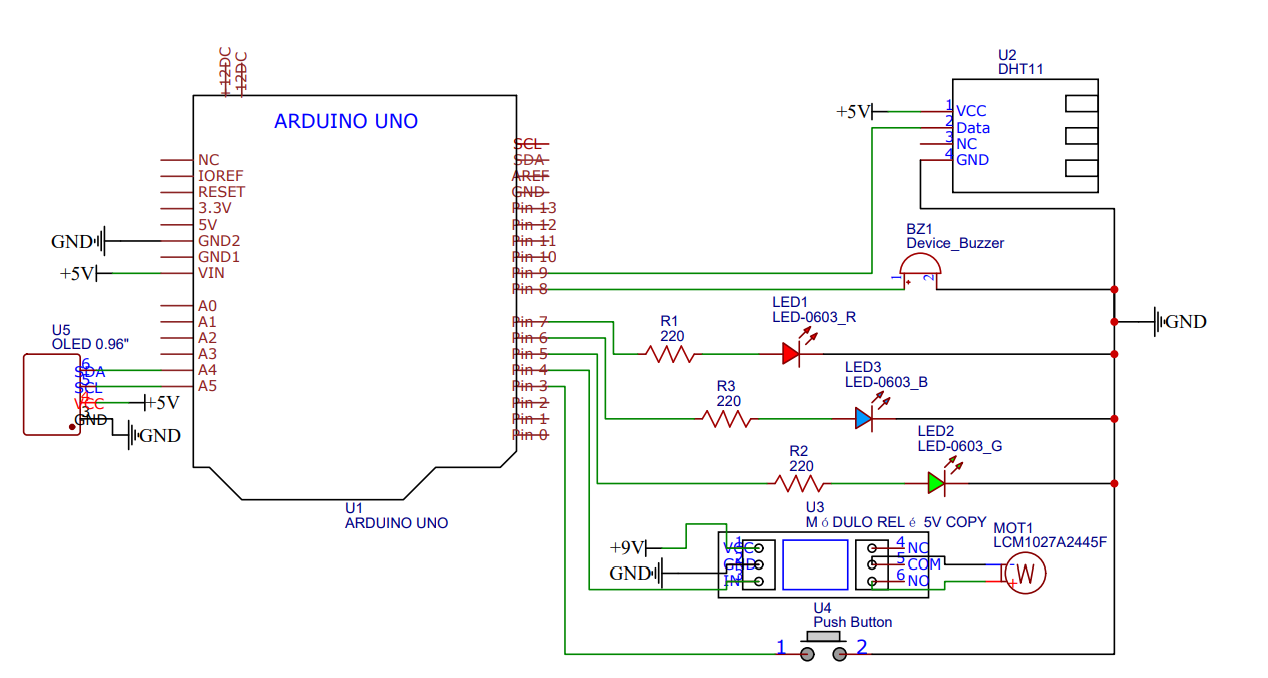
\includegraphics[width=\columnwidth]{images/Imagen_1R3.png}
                  \caption{Esquemático de Conexión Reto 3}
                  \label{fig:Imagen_1R3}
                  \end{figure}
                
            \end{itemize}
    
    \item Código Documentado

    El código propuesto documentado se encuentra registrado a continuación:
    \begin{lstlisting}[caption={Sistema de Riego Automatico con DHT11 y OLED}, label={lst:riego-automatico}]
#include <DHT.h>
#include <Adafruit_GFX.h>
#include <Adafruit_SSD1306.h>
// --- Definicion de pines ---
const int PIN_SENSOR_HUMEDAD = 2;
const int PIN_RELE           = 4;
const int PIN_LED_VERDE      = 5;
const int PIN_LED_AZUL       = 6;
const int PIN_LED_ROJO       = 7;
const int PIN_BUZZER         = 8;
const int PIN_BOTON_MANUAL   = 3;
// --- Configuracion DHT11 ---
#define DHTTYPE DHT11
DHT dht(PIN_SENSOR_HUMEDAD, DHTTYPE);
// --- Configuracion OLED ---
#define SCREEN_WIDTH 128
#define SCREEN_HEIGHT 64
#define OLED_RESET    -1
Adafruit_SSD1306 oled(SCREEN_WIDTH,
                      SCREEN_HEIGHT,
                      &Wire,
                      OLED_RESET);
// --- Umbrales de humedad ---
const int UMBRAL_SECO   = 30;
const int UMBRAL_HUMEDO = 70;
const int UMBRAL_ALARMA = 20;
const int HISTERESIS    = 5;
// --- Temporizacion ---
const long INTERVALO_LECTURA = 2000;
const long TIEMPO_MIN_RIEGO  = 5000;
// --- Enumeracion de estados ---
enum EstadoRiego
{ IDLE, REGANDO, ALARMA };
EstadoRiego estadoRiego = IDLE;
// --- Variables de control ---
float         humedadActual       = 0.0;
bool          bombaActiva         = false;
unsigned long tiempoUltimaLectura = 0;
unsigned long tiempoInicioRiego   = 0;
unsigned long tiempoBuzzer        = 0;
bool          estadoBuzzer        = false;
float leerHumedad() {
  float h = dht.readHumidity();
  if (isnan(h)) {
    Serial.println("Error DHT11");
    oled.clearDisplay();
    oled.setCursor(0, 0);
    oled.println("Error sensor");
    oled.println("DHT11 fallo");
    oled.display();
    return -1.0;
  }
  return h;
}
void activarBomba() {
  if (!bombaActiva) {
    digitalWrite(PIN_RELE, LOW);
    bombaActiva       = true;
    tiempoInicioRiego = millis();
    Serial.println("BOMBA: ACTIVADA");
  }
}
void desactivarBomba() {
  if (bombaActiva) {
    digitalWrite(PIN_RELE, HIGH);
    bombaActiva = false;
    Serial.println("BOMBA: DESACTIVADA");
  }
}
void evaluarEstadoRiego() {
  bool tiempoMinCumplido =
    (millis() - tiempoInicioRiego)
    >= TIEMPO_MIN_RIEGO;
  switch (estadoRiego) {
    case IDLE:
      if (humedadActual < UMBRAL_ALARMA){
        estadoRiego = ALARMA;
        activarBomba();
      } else if (humedadActual
                 <= UMBRAL_SECO) {
        estadoRiego = REGANDO;
        activarBomba();
      }
      break;
    case REGANDO:
      if (tiempoMinCumplido &&
          humedadActual >=
          UMBRAL_HUMEDO) {
        estadoRiego = IDLE;
        desactivarBomba();
      }
      break;
    case ALARMA:
      activarBomba();
      if (humedadActual >=
         (UMBRAL_SECO + HISTERESIS)) {
        estadoRiego = IDLE;
        desactivarBomba();
      }
      break;
  }
}
void actualizarIndicadores() {
  digitalWrite(PIN_LED_VERDE,
               estadoRiego == IDLE);
  digitalWrite(PIN_LED_AZUL,
               estadoRiego == REGANDO);
  digitalWrite(PIN_LED_ROJO,
               estadoRiego == ALARMA);
}
void gestionarBuzzerAlarma() {
  if (estadoRiego != ALARMA) {
    noTone(PIN_BUZZER);
    return;
  }
  if ((millis() - tiempoBuzzer) >= 500){
    tiempoBuzzer = millis();
    estadoBuzzer = !estadoBuzzer;
    if (estadoBuzzer)
      tone(PIN_BUZZER, 880, 250);
    else
      noTone(PIN_BUZZER);
  }
}
void verificarBotonManual() {
  if (digitalRead(PIN_BOTON_MANUAL)
      == LOW) {
    delay(50);
    if (digitalRead(PIN_BOTON_MANUAL)
        == LOW) {
      desactivarBomba();
      estadoRiego = IDLE;
      Serial.println(
        "OVERRIDE: Riego detenido");
    }
  }
}
void mostrarEnOLED() {
  oled.clearDisplay();
  oled.setTextSize(1);
  oled.setTextColor(SSD1306_WHITE);
  oled.setCursor(0, 0);
  oled.println("Sistema de Riego");
  oled.drawLine(0, 10, 127, 10,
                SSD1306_WHITE);
  oled.setTextSize(2);
  oled.setCursor(0, 16);
  oled.print("Hum: ");
  oled.print((int)humedadActual);
  oled.println("%");
  oled.setTextSize(1);
  oled.setCursor(0, 40);
  oled.print("Estado: ");
  switch (estadoRiego) {
    case IDLE:
      oled.println("OPTIMO");   break;
    case REGANDO:
      oled.println("REGANDO");  break;
    case ALARMA:
      oled.println("ALARMA!");  break;
  }
  oled.setCursor(0, 52);
  oled.print("Bomba: ");
  oled.println(bombaActiva ?
  "ON":"OFF");
  oled.display();
}
void setup() {
  Serial.begin(9600);
  dht.begin();
  pinMode(PIN_RELE,         OUTPUT);
  pinMode(PIN_LED_VERDE,    OUTPUT);
  pinMode(PIN_LED_AZUL,     OUTPUT);
  pinMode(PIN_LED_ROJO,     OUTPUT);
  pinMode(PIN_BUZZER,       OUTPUT);
  pinMode(PIN_BOTON_MANUAL,
  INPUT_PULLUP);
  digitalWrite(PIN_RELE, HIGH);
  oled.begin(SSD1306_SWITCHCAPVCC,
             0x3C);
  oled.clearDisplay();
  oled.setTextSize(1);
  oled.setTextColor(SSD1306_WHITE);
  oled.setCursor(20, 20);
  oled.println("Sistema Riego");
  oled.setCursor(25, 35);
  oled.println("Iniciando...");
  oled.display();
  delay(2000);
  oled.clearDisplay();
  Serial.println(
    "Sistema de Riego - Listo");
}
void loop() {
  unsigned long ahora = millis();
  if (ahora - tiempoUltimaLectura
      >= INTERVALO_LECTURA) {
    tiempoUltimaLectura = ahora;
    humedadActual = leerHumedad();
    if (humedadActual < 0) return;
    evaluarEstadoRiego();
    actualizarIndicadores();
    mostrarEnOLED();
    Serial.print("Humedad: ");
    Serial.print(humedadActual);
    Serial.print("% | Estado: ");
    Serial.println(estadoRiego);
  }
  gestionarBuzzerAlarma();
  verificarBotonManual();
}
\end{lstlisting}
\end{itemize}
        








